%%%%%
%%%%%  Naudokite LUALATEX, ne LATEX.
%%%%%
%%%%
\documentclass[]{VUMIFTemplateClass}

\usepackage{indentfirst}
\usepackage{amsmath, amsthm, amssymb, amsfonts}
\usepackage{mathtools}
\usepackage{physics}
\usepackage{graphicx}
\usepackage{verbatim}
\usepackage[hidelinks]{hyperref}
\usepackage{color,algorithm,algorithmic}
\usepackage[nottoc]{tocbibind}
\usepackage{tocloft}
\usepackage{makecell}
\usepackage{color}

\usepackage{titlesec}
\newcommand{\sectionbreak}{\clearpage}

\makeatletter
\renewcommand{\fnum@algorithm}{\thealgorithm}
\makeatother
\renewcommand\thealgorithm{\arabic{algorithm} algoritmas}

\usepackage{biblatex}
\bibliography{bibliografija}
%% norint pakeisti bibliografijos šaltinių numeravimą (skaitiniu arba raidiniu), pakeitimus atlikti VUMIFTemplateClass.cls 150 eilutėje

% Author's MACROS
\newcommand{\EE}{\mathbb{E}\,} % Mean
\newcommand{\ee}{{\mathrm e}}  % nice exponent
\newcommand{\RR}{\mathbb{R}}


\studijuprograma{Programų sistemų}
\darbotipas{Bakalauro baigiamasis darbas}
\darbopavadinimas{Likvidavimo algoritmo tobulinimas perviršinio užstato skolinimo protokoluose}
\darbopavadinimasantras{Improving liquidation algorithms in over-collateralized lending protocols}
\autorius{Vismantas Stonkus}
\vadovas{prof. dr. Remigijus Paulavičius}
\recenzentas{lekt. Karolis Uosis}

\begin{document}
\selectlanguage{lithuanian}

\singlespacing
\begin{titlepage}
\vskip 20pt
\begin{center}

\includegraphics[scale=0.55]{images/MIF.png}
\end{center}

\makeatletter

\vskip 20pt
\centerline{\bf \large \textbf{VILNIAUS UNIVERSITETAS}}
\vskip 10pt
\centerline{\large \textbf{MATEMATIKOS IR INFORMATIKOS FAKULTETAS}}
\vskip 10pt
\centerline{\large \textbf{\MakeUppercase{\@studijuprograma \space studijų programa}}}

\vskip 80pt
\centerline{\Large \@darbotipas}
\vskip 20pt
\begin{center}
    {\bf \LARGE \@darbopavadinimas}
\end{center}
\begin{center}
    {\bf \Large \@darbopavadinimasantras}
\end{center}
\vskip 80pt

\vskip 20pt

\centering{
    \begin{tabular}{rcp{.7\textwidth}}
        {\Large Atliko} & {\Large :} & {\Large \@autorius}\\[10pt]
        {\Large Darbo vadovas} & {\Large :} & {\Large \@vadovas}\\[10pt]
        \@ifundefined{@recenzentas}{}
            {
                {\Large Darbo recenzentas} & {\Large :} & {\Large \@recenzentas}\\[10pt]
            }
    \end{tabular}}


\vskip 110pt

\centerline{\large \textbf{Vilnius}}
\centerline{\large \textbf{\the\year{}}}

\makeatother

\newpage
\end{titlepage}
%\newgeometry{top=2cm,bottom=2cm,right=2cm,left=3cm}
\setcounter{page}{2}


\tableofcontents

\onehalfspacing

%%Santrauka
\selectlanguage{lithuanian}
\sectionnonum{Santrauka}
PERRASYTI\\
Darbe nagrinėjamos likvidacijos procesų optimizavimo galimybės perviršinio užstato skolinimo protokoluose. Tyrimo tikslas analizuoti likvidavimo strategijas, siūlomos algoritminės modifikacijos, siekiant maksimaliai padidinti likvidatoriaus pelną. Pateikiama egzistuojančių metodų apžvalga ir išsamiai analizuojamas "Optimal Fixed Spread Liquidation Strategy" algoritmas. Siūloma jo modifikacija – "pilno išeikvojimo" strategija, kuri efektyviau optimizuoja procesą, leidžiantį pilnai išnaudoti likvidacijos galimybę, neprarandant potencialaus pelno. Empiriniai duomenys iš Venus protokolo rodo, kad dauguma likvidacijų nepasiekia maksimaliai galimo pelno. Palyginus tris strategijas ("atkartoti", "iki uždarymo ribos", "pilnas išeikvojimas"), nustatyta, kad "pilno išeikvojimo" strategija generuoja iki 72\% daugiau pelno nei istorinės likvidacijos. Tai rodo, kad optimizuotos strategijos galėtų reikšmingai padidinti likvidatorių pelningumą. Šio darbo rezultatai prisideda prie skolinimo protokolų optimizavimo ekosistemos ir atveria kelią tolimesnėms analizėms, susijusioms su valiutų porų ir užstato valdymo strategijomis. Darbo tęstinumas - gilintis į tarpvalutinius keitimus ir kitas likvidacijų galimybes, didinant arbitražo algoritmų efektyvumą.\\
\textbf{Raktiniai žodžiai:} blokų graindinės, likvidacijos, arbitražas, maksimali išgaunama vertė.

\sectionnonum{Summary}
PERRASYTI\\
The study examines ways to optimize liquidation processes in over-collateralized lending protocols. The research focuses on analyzing liquidation strategies and propose algorithmic modifications to maximize the liquidator’s profit. A review of the existing methods includes a detailed analysis of the “Optimal Fixed Spread Liquidation Strategy” algorithm. A proposed modification, called "the drain" strategy, optimizes the process, enabling full utilization of the liquidation opportunity without losing its potential profit. Empirical evidence from the Venus protocol shows that most liquidations do not achieve the maximum possible profit. A comparison of three strategies (“repeat,” “up to close factor,” and “drain”) shows that "the drain" strategy generate up to 72\% more profit than historical liquidations. This demonstrates that when optimized strategies can significantly increase liquidators’ profitability. The findings of this study contribute to the ecosystem of lending protocol optimization and pave the way for further analyses related to currency pair and collateral management strategies. Future research could explore using different currencies and other liquidation opportunities to enhance the efficiency of arbitrage algorithms.\\
\textbf{Keywords:} blockchain, liquidation, arbitrage, maximal extractable value (mev).

% iliustracijų sąrašas, jei jo nereikia - ištrinkite
% \listoffigures 

%lentelių sąrašas, jei jo nereikia - ištrinkite
% \listoftables

%Žymėjimų skyrius
% \sectionnonum{Žymėjimai}
% Šis skyrius skirtas, jei yra naudojami žymėjimai. Pavyzdžiui:    
% \begin{itemize}
%     \item $\EE X$ žymi atsitiktinio dydžio $X$ vidurkį.
% \end{itemize}
%Palikti jeigu reikia

%Sutrumpinimų skyrius
\sectionnonum{Santrumpos}
\begin{tabular}{rcp{.7\textwidth}}
    {DeFi} & {} & {decentralizuotų finansų sistema, kurioje tradicinės finansinės paslaugos (paskolos, skolinimas, keitimas, draudimas ir kt.) teikiamos naudojant išmaniuosius kontraktus blokų grandinėse}
\end{tabular}
%Palikti jeigu reikia

\sectionnonum{Įvadas}
\begin{enumerate}
    \item apibrėžiamas tiriamasis objektas akcentuojant neapibrėžtumą, kuris bus išspręstas darbe,
    \item aprašomas temos aktualumas,
    \item nurodomas darbo tikslas ir uždaviniai, kuriais bus įgyvendinamas tikslas.
    \item aptariamos teorinės darbo prielaidos bei kokios metodikos ir kuriam tikslui naudojamos,
    \item apibūdinami su tema susiję literatūros ar kitokie šaltiniai,
    \item temos analizės tvarka, darbo atlikimo aplinkybės,
    \item pateikiama žinių apie naudojamus instrumentus (programas ir kt., jei darbe yra eksperimentinė dalis). Darbo įvadas neturi būti dėstymo santrauka. 
\end{enumerate}

Darbo uždavinyje\\
apibrėžiamas siekiamas rezultatas, kad būtų galimybė išmatuoti, ar tikslai ir
uždaviniai yra išspręsti, bei kokiu lygiu (vertinant kiekybę bei kokybę). Pavyzdžiui, „Atlikti literatūros
.... analizę“ nėra tinkamas uždavinys, nes nusako procesą, tačiau neapibrėžia jo rezultato. Tinkamos
uždavinio formuluotės šablonai: „Išanalizuoti literatūrą … siekiant apžvelgti ir įvertinti /… metodų
tinkamumą sprendžiamam uždaviniui/privalumus ir trūkumus sprendžiant … uždavinį/rekomenduojamas ... projektavimo gaires, šablonus ir pan.“

\subsection{Tyrimo objektas ir aktualumas}
Šiame darbe bus tiriami kriptovaliutų paskolų platformų likvidavimo mechanizmai, ypatingą dėmesį skiriant \textit{Venus} protokolui, veikiančiam \textit{Binance Smart Chain} (BSC) blokų grandinėje. Bus analizuojamos likvidavimo proceso ypatybės ir ieškoma būdų jį optimizuoti. Šio protokolo veikimo principai būdingi daugeliui kitų perviršinio užstato skolinimo sistemų. Efektyvesnis likvidavimo algoritmas, padidinantis likvidatoriaus pelną, galėtų būti pritaikytas ir kitose decentralizuotose skolinimo platformose, siekiant optimizuoti likvidacijos procesą.

\subsection{Darbo tikslas}
Darbo tikslas – sukurti ir optimizuoti likvidavimo algoritmą, kuris maksimaliai padidintų likvidatoriaus pelną.

\subsection{Uždaviniai}
Užsibrėžtam tikslui pasiekti keliami šie uždaviniai:
\begin{enumerate}
  \item Apžvelgti esamus perviršinio užstato skolinimo protokolus, išanalizuoti jų veikimo principus ir palyginti juos su \textit{Venus} protokolu. Kadangi daugelis skolinimo protokolų kriptovaliutų ekosistemoje veikia panašiai, jei ši prielaida pasitvirtins, gauti rezultatai galės būti pritaikyti ir kituose protokoluose.
  \item Išsamiai išnagrinėti \textit{Venus} protokolo likvidavimo mechanizmą.
  \item Sukurti ir/arba modifikuoti efektyvesnį likvidavimo algoritmą. Šiuo uždaviniu siekiame praplėsti kursiniame darbe pristatytas likvidavimo strategijas („atkartoti“, „iki uždarymo ribos“, „pilnas išeikvojimas“) papildant jas keturiomis naujomis strategijomis, kurios atsisako fiksuotų skolos ir užstato valiutų porų:
  \begin{itemize}
    \item \textbf{Didžiausia skola} (single largest borrow) – grąžinama ta skolos valiuta, kurios suma yra didžiausia. Užstatas pasirenkamas iš tos pačios valiutos, jei užstato kiekis yra pakankamas, kitu atveju – valiuta, kurios vertė skolininko portfelyje didžiausia.
    \item \textbf{Nuo mažiausio likvidavimo slenksčio} (from smallest collateral factor) – pirmiausia pasirenkamos užstato valiutos su mažiausiu likvidavimo slenksčiu, o paskutinė likvidacija vykdoma pagal „Didžiausios skolos“ strategiją.
    \item \textbf{Nuo didžiausio likvidavimo slenksčio} (from largest collateral factor) – analogiška ankstesnei strategijai, tačiau prioritetas teikiamas užstato valiutoms su didžiausiu likvidavimo slenksčiu.
    \item \textbf{Vienodos valiutos} (same tokens) – atliekamos „Pilno išeikvojimo“ strategijos likvidacijos tik toms valiutoms, kurios yra tiek užstatytos, tiek pasiskolintos. Ši strategija leidžia sumažinti valiutų keitimo riziką ir likvidumo problemas.
  \end{itemize}
  \item Palyginti sukurtas strategijas tarpusavyje bei su istorinėmis likvidacijomis.
  \item Apibendrinti rezultatus ir pateikti išvadas bei rekomendacijas. Bus bandoma atsakyti į šiuos klausimus:
  \begin{itemize}
    \item Ar „Nuo mažiausio likvidavimo slenksčio“ strategija yra pelningiausia likvidatoriui? Ši hipotezė grindžiama skolinimosi pajėgumo formule: jis priklauso nuo užstato valiutų verčių ir jų likvidavimo slenksčių sandaugų sumos. Tarkime, kad skolininkas yra užstatęs dvi vienodos vertės valiutas, tačiau vienos valiutos likvidavimo slenkstis yra 50\%, o kitos – 90\%. Užstatas su mažesniu likvidavimo slenksčiu mažiau prisideda prie skolinimosi pajėgumo nei užstatas su didesniu slenksčiu. Todėl likviduojant pirmiausia mažesnio slenksčio užstatą, mažiau paveikiamas bendras skolinimosi pajėgumas, o tai gali lemti didesnį likvidatoriaus pelną.
    \item Ar „Nuo didžiausio likvidavimo slenksčio“ strategija, kuri veikia priešingai nei optimalios strategijos, rodys mažesnį pelną likvidatoriui?
    \item Ar „Vienodos valiutos“ strategija sustiprina „Pilno išeikvojimo“ strategijos pagrįstumą, nes eliminuoja valiutų konvertavimo riziką ir likvidumo trūkumą vykdant arbitražą didelėmis sumomis?
  \end{itemize}
\end{enumerate}

\subsection{Metodai (ir prielaidaos ir instrumentai)}
\{Cia papasakoti, kad likvidacijos pelningumas yra vertinimas pasinaudojant tuometinemis valiutu vertemis is tam tikro\}
Pirmiems dviem užduotims bus nagrinėjimas paviešintas protokolų kodas.
Kaip trecia
kaip ketvirta


PERRASYTI
Kriptovaliutos, kaip sparčiai auganti finansinė sritis, yra populiarus objektas spekuliantams, kurie siekia pasipelnyti iš šių valiutų vertės svyravimų. Nepaisant didelių pelningumo galimybių, investavimas į kriptovaliutas neatsiejamas nuo rizikos, kad valiutos vertė gali smarkiai nukristi, dėl ko investuotojas gali prarasti dalį ar net visą pradinę investiciją. Siekiant maksimalaus pelno ir minimalios rizikos yra taikomi automatiniai arbitražo algoritmai. Šie algoritmai analizuoja kriptovaliutų rinkos svyravimus ir automatiškai vykdo sandorius, leidžiančius pasipelnyti iš mažiausių kainų skirtumų tarp skirtingų biržų.

Šiame darbe dėmesys yra sutelktas į likvidacijos procesą ir jo integravimą į esamus automatinio arbitražo algoritmus. Darbo tikslas – analizuoti ir palyginti skirtingas likvidavimo strategijas perviršinio užstato skolinimo protokoluose, siekiant sukurti ir optimizuoti algoritmą, kuris maksimaliai padidintų likvidatoriaus pelną, efektyviai išnaudojant rinkos svyravimus ir automatizuoto arbitražo galimybes.

Tam, kad darbo tikslas būtų įgyvendintas buvo išsikelti uždaviniai:
\begin{enumerate}
    \item Apžvelgti esamus perviršinio užstato skolinimo protokolus bei jų veikimo principus.
    \item Išnagrinėti likvidavimo proceso mechanizmą.
    \item Sukurti ar pamodifikuoti algoritmą, skirtą efektyviam likvidavimo strategijų vykdymui automatizuoto arbitražo sąlygomis.
    \item Palyginti sukurtą algoritmą su egzistuojančiais sprendimais, įvertinant pelningumą.
\end{enumerate}

Darbo struktūra yra sudaryta iš kelių pagrindinių skyrių. Pirmajame skyriuje pristatoma, kas yra arbitražas, siekiant suteikti teorinį pagrindą. Antrajame skyriuje aptariamos likvidacijos, jų svarba ir galimybės kriptovaliutų pasaulyje. Trečiajame skyriuje analizuojamos skirtingos likvidacijų strategijos, o ketvirtajame skyriuje pateikiami tyrimo rezultatai, įskaitant pelningumo skaičiavimus, strategijų realizacijos pavyzdžius ir duomenų analizę. Darbas užbaigiamas rezultatais ir išvadomis, kurios apibendrina pagrindines darbo įžvalgas.

% \section{Medžiagos darbo tema dėstymo skyriai}
% pradiniai duomenys, jų analizės ir apdorojimo metodai, sprendimų įgyvendinimas, gautų rezultatų apibendrinimas.

\section{Kas yra arbitražas}
Arbitražas yra finansinė strategija, grindžiama ekonominių skirtumų išnaudojimu tarp dviejų ar daugiau rinkų, siekiant gauti pelną be jokios rizikos ar su minimalia rizika. Paprastai tariant, tai yra praktika, kai investuotojai perka tam tikrus finansinius instrumentus, tokius kaip prekės ar valiutos pigesnėje rinkoje, ir tuoj pat pardavinėja juos brangesnėje rinkoje, gaudami pelną iš šio kainų skirtumo.

Vienas esminių arbitražo principų yra reliatyvumas -- investuotojai renkasi referencinę valiutą, kurios vertę jie laiko stabilia ir dirba siekdami padidinti šios valiutos kiekį. Pavyzdžiui, jei arbitražininkas laiko eurą stabilia valiuta, jis perka ir parduoda kitas valiutas arba kitokį turtą, tikėdamasis gauti kuo didesnį pelną eurais.

Paprasčiausias arbitražas susideda iš kainų skirtumų tarp dviejų rinkų. Tai pasiekiama konvertuojant stabilų turto vienetą į kitą valiutą pagal kursą $P_1$ ir vėliau konvertuojant šią valiutą atgal į pradinį stabilų turto vienetą kursu $P_2$, kur $P_1 \cdot P_2 > 1$. Šią pagrindinę idėją galima plėtoti ir modifikuoti įvairiais būdais:

\begin{itemize}
    \item įtraukti tarpinius konvertavimo žingsnius, sudarant ilgesnę operacijų grandinę, siekiant išnaudoti kainų skirtumus biržose, kuriose nėra tiesioginio konvertavimo kelio iš ar į stabiliąją valiutą;
    \item pradėti arbitražą ne vien tik su viena stabiliąja valiuta, bet su keliomis. Taip galima efektyviau išnaudoti turimą kapitalą, nes skirtingos stabilių valiutų pozicijos gali suteikti daugiau lankstumo ir galimybių reaguoti į kainų skirtumus įvairiose biržose;
    \item išskaidyti valiutos konvertavimą į kitą per kelias biržas, siekiant išvengti didelio kainų svyravimo vienoje biržoje;
    \item konvertuoti vieną turto vienetą į kelias skirtingas valiutas vienoje tranzakcijoje dėl tam tikrų platformų galimybių;
    \item pasiskolinti kapitalą iš biržos su sąlyga, kad skola bus grąžinta per arbitražo procesą, taip panaikinant reikalavimą turėti pradinį kapitalą.
\end{itemize}

Efektyviausia arbitražo ypatumus pateikti pasinaudojant grafais. Pavyzdžiui, grafe, kur mazgai reprezentuoja savininkų sąskaitas (tradicinių valiutų atveju) arba piniginės adresus (kriptovaliutų atveju), o kryptinės briaunos – valiutų ar kriptovaliutų persiuntimus tarp jų, aiškiai matoma turtų judėjimo dinamika ir galimos arbitražo pelno galimybės. 

\begin{figure}[H]
    \centering
    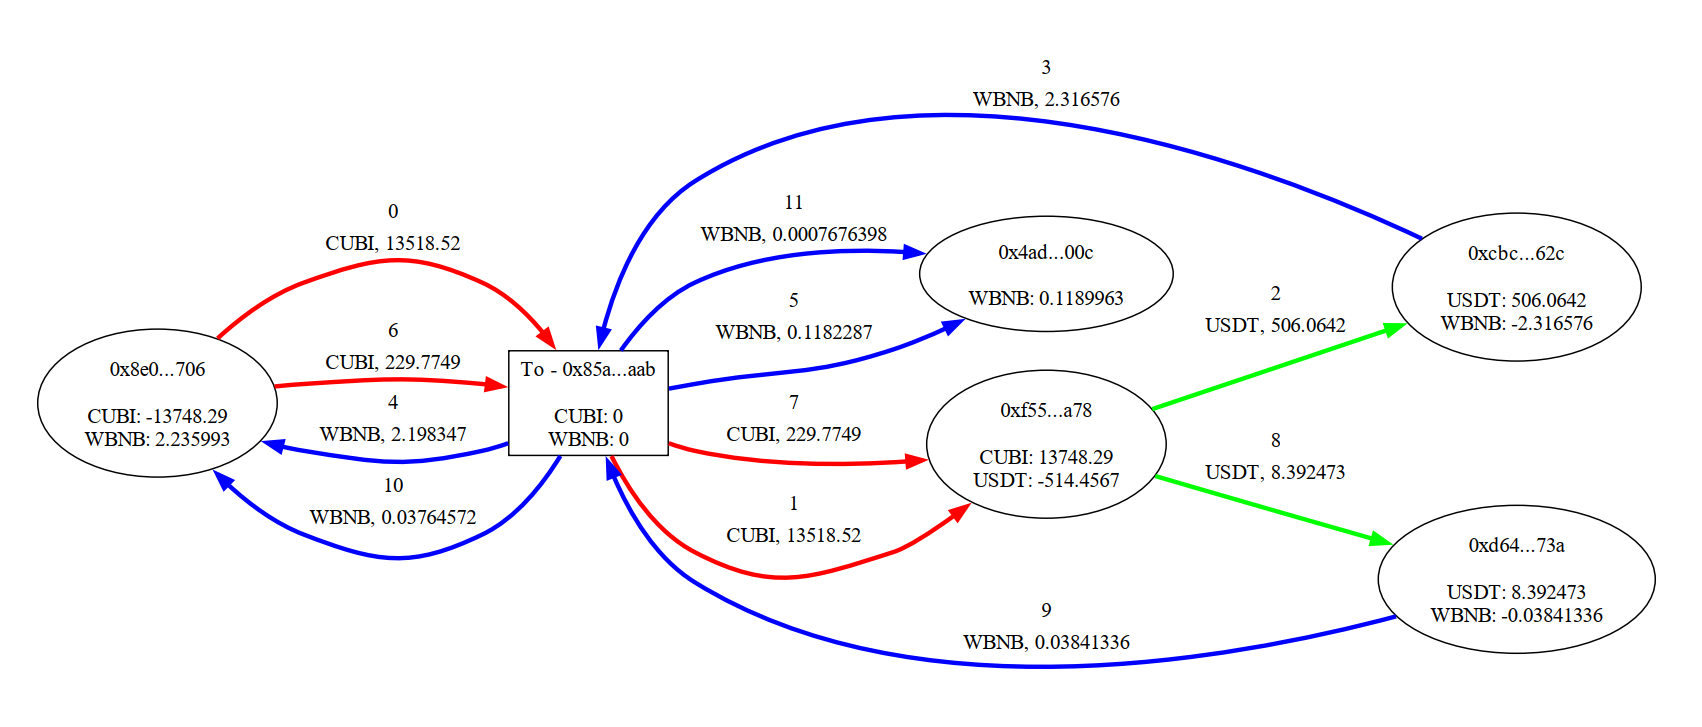
\includegraphics[scale=0.3]{img/arb1.png}
    \caption{Arbitražo vizualizacija: lėšų pervedimai ir galutinis pelnas – 0,11899 WBNB}
    \label{img:chess-minimax-2}
\end{figure} 

\ref{img:chess-minimax-2} pav. pateikta arbitražo vizualizacija kriptovaliutų atveju. Matome 12 pavedimų tarp skirtingų piniginių adresų (numeracija prasideda nuo 0). Šiuo atveju adresas 0x85a..aab yra pradinis kontrakto adresas, kuris buvo iškviestas tranzakcijoje. Iš viso tranzakcijoje dalyvauja 4 rinkos, kuriose galima konvertuoti valiutų poras:

\begin{itemize}
    \item 0x8eo..706 -- CUBI - WBNB
    \item 0xf55..a78 -- CUBI - USDT
    \item 0xcbc..62c -- USDT - WBNB
    \item 0xd64..73a -- USDT - WBNB
\end{itemize}

Adresas 0x4ad..00c šiuo atveju yra tik pelno piniginė, kurioje tranzakcijos pabaigoje atsiranda papildomi 0,11899 WBNB valiutos.

Kiekviename mazge taip pat pažymėtos valiutos ir jų kiekiai, nurodantys galutinį valiutos skirtumą po tranzakcijos. Pavyzdžiui, rinkoje 0x8eo..706 valiuta WBNB -> CUBI buvo konvertuota du kartus, kur iš viso į rinką įdėta 2,235993 WBNB, o išimta 13748,29 CUBI.

Tranzakciją galima suskirstyti į dvi dalis su pavedimais 0-5 ir 6-11. Pirmuosiuose penkiuose pavedimuose (0-4) atliekamas ratas: pradžioje trumpam pasiskolinama CUBI, tada ji iškeičiama į USDT, o po to -- į WBNB. Trečiuoju pavedimu gaunama daugiau valiutos, nei reikia skolai grąžinti ketvirtuoju pavedimu. Todėl perviršis lieka kaip pelnas, kuris penktuoju pavedimu persiunčiamas į pelno piniginę. Panašiai vyksta ir su pavedimais 6-11, tačiau antrojoje dalyje naudojama kita USDT-WBNB rinka, o apskritai keičiamų valiutos kiekių dydžiai yra mažesni.

\section{Likvidacijos}

\{Reiktu parasyti kodel cia rasom teksta ir kodel dedikuojam tiek daug puslapiu sitai minciai\}

Koks yra sios analizes tikslas? Suprasti apie defi paskolu platformas ir kuo ju likvidavimo procesas issiskiria nuo tradiciniu finansu sistemu.

\subsection{Tradicinės paskolų platformos}
Paskolų platformos – tai sistemos, kuriose vartotojai gali skolintis ar skolinti pinigus kitiems vartotojams. Tradicinėse bankinėse sistemose bankas veikia kaip tarpininkas tarp skolintojo ir skolininko. Panašiai veikia ir kredito unijos, kuriose nariai vieni kitiems suteikia paskolas per bendrą fondą.

\subsubsection{Veiklos principas}
\begin{itemize}
    \item \textbf{Skolintojai}: asmenys ar įmonės, turintys perteklinių lėšų, kurias jie norėtų investuoti, kad gautų grąžą kaip palūkanas.
    \item \textbf{Skolininkai}: asmenys ar įmonės, kuriems reikia lėšų įvairiems tikslams – pradėti verslą, finansuoti projektą, pirkti prekę ir pan.
\end{itemize}

Skolintojai įneša savo lėšas į platformą, o skolininkai pateikia prašymus dėl paskolų. Platforma tada suderina šiuos du suinteresuotus šalių poreikius. Priklausomai nuo platformos ir paskolos tipo, gali būti reikalaujama, kad skolininkai užstatytų tam tikrą turto dalį kaip garantiją.

\subsubsection{Likvidacijos tradicinėse sistemose}
Tradicinėse finansų sistemose likvidacija vyksta tuomet, kai skolininkas nesugeba įvykdyti savo įsipareigojimų grąžinti paskolą. Tokiu atveju kredito įstaiga (bankas ar kredito unija) gali pradėti priverstinį skolų išieškojimo procesą, kuris dažnai apima užstato realizavimą.

Procesas dažnai prasideda nuo skolininko įspėjimo apie neįvykdytą mokėjimą. Jeigu situacija nesikeičia, kreditorius gali inicijuoti teisinį procesą: kreiptis į antstolius arba teismą dėl turto arešto ir pardavimo. Užstatas, pavyzdžiui, nekilnojamasis turtas ar transporto priemonė, įvertinamas ir parduodamas aukcione arba per kitus kanalus.

Gautos lėšos naudojamos skolos padengimui. Jeigu užstato realizavimo suma viršija skolos vertę, likutis grąžinamas skolininkui. Priešingu atveju, jei skolos likutis išlieka, skolininkas lieka skolingas likusią sumą. Procesas yra ilgesnis nei automatizuotose sistemose, tačiau suteikia galimybę ginčams spręsti ir apsaugoti abi puses teisinėmis priemonėmis.

\subsection{Kriptovaliutų paskolų platformos}
Šiuolaikinėse paskolų platformose populiarėja kriptovaliutų paskolų modelis, kuriame operacijos atliekamos naudojant kriptovaliutas arba kitą kriptoturtą kaip užstatą. Skolinimo ir grąžinimo procesai šiose platformose vykdomi naudojant išmaniuosius kontraktus (angl. \textit{smart contracts}). Tokios platformos priklauso decentralizuotų finansų (angl. \textit{Decentralized Finance}, \textit{DeFi}) sistemai – tai finansinių paslaugų ekosistema, veikianti be tarpininkų, pagrįsta blokų grandinės technologija ir automatizuota išmaniųjų kontraktų pagalba.

Viena iš svarbiausių šių platformų savybių yra tai, kad skolininkai privalo pateikti užstatą, kuris viršija paimtos paskolos vertę. Kriptovaliutų pasaulyje tokia perviršinio užstato sistema yra būtina, nes leidimas skolintis daugiau nei pateikto užstato vertė atvertų kelią reikšmingam išnaudojimui. Jei būtų galima pateikti mažai užstato ir gauti didelę paskolą, tai sukeltų didelę riziką platformai, nes skolininkai galėtų nesąžiningai išnaudoti šią galimybę, o skolintojai patirtų didžiulius nuostolius. Todėl perviršinio užstato reikalavimas yra esminis saugumo mechanizmas, užtikrinantis stabilumą ir patikimumą šiose finansinėse sistemose.\cite{whatisdefiliquidation}

Dar viena kriptovaliutų paskolų platformų ypatybė -- tai valiutų vertės nustatymo procesas, kuris yra atliekamas naudojant orakulus. Orakulai yra išoriniai informacijos tiekėjai, kurie pateikia duomenų srautą naudojantis išmaniaisiais kontraktais. Šie kontraktai yra periodiškai atnaujinami per privilegijuotas \textit{blockchain} tranzakcijas. Šios tranzakcijos nustato tam tikros valiutos vertę, užtikrindamos sklandų ir patikimą platformos veikimą.

\subsubsection{Kodėl žmonės skolinasi per kriptovaliutų paskolų platformas?}

\begin{enumerate}
    \item \textbf{Kapitalo prieinamumas neparduodant turto}: skolinantis per kriptovaliutų platformas, galima gauti lėšų neparduodant turimų kriptovaliutų, taip išvengiant galimų mokesčių ir toliau dalyvaujant rinkos augime \cite{kriptovaliutosio}.
    \item \textbf{Greitas ir paprastas procesas}: kriptovaliutų paskolos dažnai suteikiamos greičiau ir su mažiau biurokratijos nei tradicinės bankų paskolos, nes nereikalaujama kredito istorijos patikrinimo \cite{targettrend}.
    \item \textbf{Trumpasis pardavimas}: dar angliškai vadinamas \textit{shorting}. Kriptovaliutų skolinimo platformos leidžia naudotojams skolintis kriptovaliutas, kurias jie vėliau parduoda dabartine rinkos kaina tikėdamiesi kainų kritimo ateityje. Kainai nukritus yra nuperkamas tas pats kiekis valiutos, kiek buvo pasiskolinta, ir iš karto gražinama skola. Šis metodas leidžia investuotojams uždirbti iš rinkos kainų svyravimų net ir krintant kainoms. Pavyzdžiui, investuotojas gali užstatyti savo ETH, pasiskolinti BTC, parduoti BTC už \$30000, tariant, kad einamuoju metu yra tokia kaina, ir vėliau nusipirkti už \$25000, tariant, kad po kažkiek laiko kaina nukrito, grąžindamas skolą ir pasilikdamas \$5000 pelno.
    \cite{shortinimas}.
\end{enumerate}

\subsubsection{DeFi likvidacijų palyginimas su tradicinę finansų sistemą}
DeFi likvidacijos procesas skiriasi nuo tradicinio likvidavimo keliais esminiais aspektais, kurie yra svarbūs norint suprasti, kodėl šiose sistemose leidžiama įtraukti daugiau dalyvių – trečiąsias šalis, atliekančias likvidaciją\cite{whatisdefiliquidation}:

\begin{itemize}
    \item \textbf{Automatizavimas:} DeFi likvidacijos paprastai yra automatizuotos naudojant išmaniuosius kontraktus, todėl nereikia žmogaus įsikišimo. Tradicinėse finansų sistemose maržos reikalavimas (angl. \textit{margin call}) dažnai reikalauja skolininko ar tarpininko rankinio veiksmo.
    
    \item \textbf{Skaidrumas:} DeFi likvidacija yra visiškai skaidri – visos tranzakcijos vyksta viešoje blokų grandinėje. Tradicinėse finansų sistemose likvidacijos detalės gali būti sunkiau prieinamos ar nematomos plačiajai visuomenei.
    
    \item \textbf{Decentralizacija:} DeFi veikia be tarpininkų – kriptovaliutų likvidacijos vykdomos tiesiogiai per kodo logiką. Tradicinėse finansų sistemose likvidacijas valdo brokeriai arba finansinės institucijos.
\end{itemize}

Kai skolininko užstato vertė krinta žemiau likvidavimo ribos (angl. \textit{liquidation threshold}), pagal protokolą bet kam leidžiama atlikti likvidaciją. Per likvidacijos procesą užstatas (angl. \textit{collateral}) yra parduodamas, dažnai su tam tikra nuolaida, mainais į valiutą, kurią skolininkas pasiskolino. \cite{venusliquidations}

\subsubsection{Protokolai}

Yra daugybė paskolų protokolų, veikiančių įvairiuose \textit{blockchain} tinkluose, kurie suteikia vartotojams galimybę skolintis ir skolinti decentralizuotai. \ref{tab:sample_table} lentelėje pateikiami keli populiariausi šių protokolų pavyzdžiai. 

\begin{itemize}
  \item \textbf{Blokų grandinės} – išvardijami \textit{blockchain} tinklai, kuriuose veikia atitinkamas protokolas. Paskolų mechanizmas tarp tinklų gali skirtis dėl tinklo subtilybių, tačiau pagrindiniai procesai išlieka tokie pat tam pačiam protokolui.
  \item \textbf{Bendra užrakinta vertė (Total Value Locked)} – atspindi platformos bendrą turto vertę įdėtą naudotojų. Tai svarbus rodiklis, leidžiantis įvertinti protokolo populiarumą ir pasitikėjimą. Paskolų platformų kontekste, ši vertė nurodo bendrą užstato sumą, iš kurios kaupiamos palūkanos už paskolintą turtą.
  \end{itemize}
  
Iš lentelės matome, kad Aave yra vienas iš populiariausių ir labiausiai paplitusių paskolų protokolų, veikiantis daugybėje \textit{blockchain} tinklų ir turintis didžiausią bendrą užrakintą vertę – \$22,112 milijardų. Šis protokolas išsiskiria savo plačia integracija ir stipriu vartotojų pasitikėjimu.


\begin{table}[H]
  \centering
  \caption{Paskolų protokolų palyginimas \cite{LikvidacijuProtokolai}}
  \begin{tabular}{|l|p{7cm}|p{5cm}|}
  \hline
  \textbf{Pavadinimas}       & \textbf{Blokų grandinės}                                                                 & \makecell{\textbf{Bendra užrakinta vertė} \\ \textbf{(Total Value Locked)}} \\ \hline
  Aave                      & Ethereum, Arbitrum, Avalanche, Polygon, Base, Optimism, Scroll, BSC, Gnosis, Metis, ZKsync Era, Fantom, Harmony & \$22,112B \\ \hline
  JustLend                  & Tron                                                                                  & \$7,282B  \\ \hline
  Spark                     & Ethereum, Gnosis                                                                      & \$5,391B  \\ \hline
  Compound Finance          & Ethereum, Arbitrum, Base, Optimism, Polygon, Scroll                                   & \$3,051B  \\ \hline
  Morpho                    & Ethereum, Base                                                                        & \$2,930B  \\ \hline
  Kamino Lend               & Solana                                                                                & \$2,126B  \\ \hline
  Venus                     & BSC, ZKsync Era, Arbitrum, opBNB, Ethereum                                            & \$1,938B  \\ \hline
  Avalon Labs               & CORE, Bitlayer, Taiko, BSC, Merlin, BOB, Mode, BSquared, ZetaChain, Kaia, Arbitrum, Ethereum, Base, IoTeX, Scroll, Mantle, Zircuity & \$1,134B  \\ \hline
  Fluid Lending             & Ethereum, Arbitrum, Base                                                              & \$622,38M \\ \hline
  Benqi Lending             & Avalanche                                                                             & \$511,67M \\ \hline
  NAVI Lending              & Sui                                                                                   & \$476,31M \\ \hline
  Suilend                   & Sui                                                                                   & \$468,55M \\ \hline
  Marginfi Lending          & Solana                                                                                & \$453,06M \\ \hline
  \end{tabular}
  \label{tab:sample_table}
\end{table}

\subsubsection{Venus platforma}

% Šiame darbe toliau yra analizuojamas \textit{Venus} protokolas ir jo istorinės likvidacijos. Nors ši platforma nėra didžiausia, jos likvidavimo mechanizmai yra panašūs į daugelio kitų kriptovaliutų paskolų platformų, todėl darbo rezultatai gali būti laikomi reprezentatyviais platesnei šios srities ekosistemai. \textit{Venus} protokolas pasirinktas dėl autoriaus asmeninio susipažinimo su jo veikimu ir ilgametės patirties pagrindiniame jo \textit{blockchain} tinkle – \textit{Binance Smart Chain (BSC)}.

Šiame darbe toliau yra analizuojamas \textit{Venus} protokolas ir jo istorinės likvidacijos. Nors ši platforma nėra didžiausia, jos likvidavimo mechanizmai yra panašūs į daugelio kitų kriptovaliutų paskolų platformų. Tai bus detaliau parodyta skyriuje \ref{sec:venus_mechanizmas}

\textit{Venus} protokolas pasirinktas dėl autoriaus asmeninio susipažinimo su jo veikimu ir ilgametės patirties pagrindiniame jo \textit{blockchain} tinkle – \textit{Binance Smart Chain (BSC)}.

\subsubsection{Arbitražo potencialas}
Iš esmės, likvidaciją galima laikyti tam tikra rinka, suteikiančia galimybę konvertuoti vieną valiutą į kitą. Likvidacija paprastai yra pelninga likviduotojams, nes pasiskolinta valiuta yra iškeičiama į užstatą, kurio vertė dažnai viršija grąžintos paskolos sumą – taip likvidatoriams sukuriama finansinė paskata veikti. Ši procedūra yra nepalanki skolininkui, nes jis priverstinai praranda dalį arba visą savo užstatą. Skolintojams likvidacija naudinga tuo, kad užtikrina paskolos grąžinimą net ir tuomet, kai skolininkas pats to padaryti nesugeba. Todėl likvidacijos procesas yra naudingas likviduotojams ir skolintojams, tačiau nuostolinga skolininkui.

Jeigu valiuta, kuria reikia grąžinti skolą, yra nestabili iš likvidatoriaus perspektyvos, galima konvertuoti turima kapitalą iš stabilios valiutos į skolinamąją valiutą. Panašiai, užstato valiutą galima konvertuoti į stabilų piniginį vienetą per tam tikras valiutų keitimo operacijas kitose rinkose. Tokiu atveju, arbitražo sistema tampa itin vertinga, nes ji gali automatizuoti valiutos konversijos procesą ir rasti efektyviausią būdą konvertuoti iš valiutos A į valiutą B, tuo pačiu užtikrinant, kad likvidatorius gaus maksimalų pelną.

Taigi, jeigu turime algoritmą, kuris sugeba aptikti arbitražo galimybes iš tam tikros rinkų aibės, šią aibę galima papildyti likvidacijos rinkomis, leidžiant likvidatoriams bandyti pasipelnyti iš likvidacijų su minimalia ar net be rizikos. Tačiau likvidatoriai gali susidurti su rizikomis -- pavyzdžiui, būti aplenktiems kitų likvidatorių arba mokėti mokesčius už bandymus atlikti likvidaciją be sėkmingo likvidavimo dėl klaidos ar būsenos pasikeitimo, kuri nebeleistų atlikti valiutų konvertavimo. Šios rizikos yra aktualios ir paprastesniems arbitražo scenarijams tarp rinkų.

\section{Venus protokolo likvidavimo mechanizmas}
\label{sec:venus_mechanizmas}

\textcolor{red}{
\{Koks tikslas sito skyriaus? Kokius klausimus norim atsakyti?\}
Norim išsamiai išnagrinėti Venus protokolo likvidavimo mechanizmą.
Palyginti kitus paskolu platformu mechanizmus su Venus ir parodyti, kad tolimesni algoritmai gali buti pritaikyti kitose platformose.
}

Šiame skyriuje siekiama išsamiai išanalizuoti \textit{Venus} protokolo likvidavimo mechanizmą, suprasti jo veikimo principus bei išskirti pagrindinius parametrus, lemiančius likvidacijos eigą. Nors pasirinktas konkretus protokolas, analizė nėra skirta tik jam – šiuo tyrimu taip pat siekiama įvertinti, kiek \textit{Venus} modelis yra atstovaujantis platesnei kriptovaliutų paskolų platformų ekosistemai. Lyginant su kitais protokolais, bus siekiama pagrįsti, kad tolimesni šiame darbe siūlomi algoritmai gali būti taikomi ir kitose panašaus tipo decentralizuotose skolinimo sistemose.

\subsection{Sąvokos}
\begin{itemize}
  \item \textbf{Pozicija (angl. \textit{position})}: rinkinys kelių užstatų ir paskolų, suskirstytų pagal valiutą, kuriuos valdo vienas naudotojas.
  \item \textbf{Likvidacijos paskata}: priedas arba nuolaida, kurią likvidatorius gali gauti, likviduodamas užstatą.
  Šis skirtumas skatina likvidatorius veikti nedelsiant, kai paskola peržengia likvidavimo slenkstį. \textit{Venus} atveju tai yra 10\% gražinamos valiutos vertės.
  \item \textbf{Paskolos ir užstato santykis (angl. \textit{loan to value, LTV})}: procentinė dalis, kuria užstato vertė įtraukiama į skolinimosi pajėgumą. Kiekviena valiuta turi atskirą vertę (paprastai nuo 60\% iki 90\%). 
  \item \textbf{Uždarymo riba (angl. \textit{close factor, CF})}: maksimali skolos dalis, kuri leidžiama būti grąžinta vienos likvidacijos metu. Vertė yra bendra visam protokolui, mūsų atveju 50\%.
  \item \textbf{Skolinimosi pajėgumas (angl. \textit{borrowing capacity, BC})}: apibrėžia bendrą vertę, kurią skolininkas gali pasiskolinti, atsižvelgiant į jo užstato sumą.
    \[
    \text{BC} = \sum_{i} \bigl(\text{Užstato vertė}_{i} \times LT_{i}\bigr), \quad \text{kur } i \text{ žymi } i\text{-ąją valiutą pozicijoje}
    \]
  \item \textbf{Sveikumo koeficientas (angl. \textit{health factor, HF})}: matuoja pozicijos būklę, apibrėžiamą kaip skolinimosi pajėgumo ir esamų skolų santykį. Jeigu sveikumo koeficientas mažesnis negu 1, skolininkas tampa likviduojamas.
  \[
  \text{HF} = \frac{\text{BC}}{\sum_{i} \text{Skolos vertė}_{i}}
  \]
\end{itemize}

\subsection{Likvidacijos ypatumai}

Skolininkui tapus likviduojamu, yra daugybė pasirinkimų, kaip vykdyti jo pozicijos likvidavimą. Likvidavimo proceso metu būtina pasirinkti konkrečią užstato ir paskolos valiutų porą, kurioje paskolos valiuta yra grąžinama, o užstato valiuta paimama iš skolininko. Taip pat, nustatomas grąžintinos sumos dydis. Svarbu pabrėžti, jog atlikus nedidelę likvidaciją, skolininkas gali išlikti likviduojamas, tai reiškia, kad likvidavimo procesas gali būti vykdomas kelis kartus.

Svarbu pažymėti, kad likvidavimo metu protokolas leidžia likviduoti didesnį valiutos kiekį, nei būtina skolininko pozicijai subalansuoti. Tarkime:
\begin{itemize}
  \item skolininkas yra pateikęs \$2000 vertės BTC (bitkoino) valiutą kaip užstatą;
  \item BTC valiutos paskolos ir užstato santykis (\textit{LTV}) yra 80\%;
  \item skolininkas yra pasiskolinęs 1650 USDT valiutos, kuri atitinka JAV dolerį.
\end{itemize}

Toliau \ref{tab:likvidacijos_pav} lentelėje matyti, kaip šios vertės kinta po skirtingo dydžio likvidacijų.
Pirmuoju variantu grąžinama \$417, po kurios skolininko sveikumo koeficientas pakyla virš 1, todėl
skolininko pozicija nustoja būti likviduojama.
Antruoju variantu grąžinama maksimali suma, kiek leidžiama, kai uždarymo riba lygi 50\%.
Šiuo atveju pozicija taip pat tampa „sveika“, tačiau skolininkas patiria didesnį nuostolį, o likvidatorius – didesnį pelną.

\begin{table}[h!]
  \centering
  \begin{tabular}{lccccc}
  \hline
  \textbf{Būsena} 
  & \textbf{Užstato vertė}
  & \textbf{Skolos vertė}
  & \textbf{BC}
  & \textbf{HF}
  & \makecell{\textbf{Pelnas likvidatoriui /}\\ \textbf{nuostolis skolininkui}} \\ 
  \hline
  Pradinė                
  & 2000      
  & 1650      
  & 1600      
  & 0,97    
  & --         \\
  
  Po \$417 likvidacijos  
  & 1541,3    
  & 1233      
  & 1233,04   
  & 1,00003   
  & 41,7       \\
  
  Po \$825 likvidacijos  
  & 1092,5    
  & 825       
  & 874       
  & 1,06      
  & 82,5       \\
  \hline
  \end{tabular}
  \caption{Pavyzdinė užstato, skolos ir sveikumo koeficiento kaita po likvidacijos}
  \label{tab:likvidacijos_pav}
  \end{table}

Likvidatoriams yra naudinga grąžinti kuo didesnę skolą už skolininką, nes už grąžintą paskolos valiutą atlyginama tokios pačios vertės užstatu, be to, papildomai suteikiama 10\% užstato kaip paskata. Likvidatorių procesą riboja du pagrindiniai dalykai: skolininko užstato dydis ir maksimali uždarymo riba.

Likvidavimo proceso kintamųjų įvairovė lemia sudėtingą optimizavimo problemą, kuri reikalauja ne tik išsamaus problemos modelio, bet ir kūrybingų algoritminių sprendimų.

\{Parodome, kad galime likviduoti daugiau nei leidziama vienu\}

\subsection{Panašumai su kitais protokolais}
Parodome, kad panasus dalykai yra ir aave'eje ir kituose dideliuose

\section{Skirtingos likvidacijų strategijos}

\subsection{Naivus algoritmas}

Paprasta likvidavimo algoritmo idėja gali būti tokia: pasirenkama paskolos valiuta, kuriai skolininkas turi didžiausią įsipareigojimą, ir užstato valiuta, kurios kiekis yra didžiausias. Tada stengiamasi grąžinti pusę paskolos arba tiek, kad būtų išnaudotas visas skolininko užstatas parinktai valiutai. Kadangi praktikoje dažniau pasiekiama uždarymo riba, o ne skolininko užstato ribojimas, šiai strategijai suteikiame konkretesnį pavadinimą – \textbf{iki uždarymo ribos}.

Pavyzdžiui, \ref{tab:naivus_pav} lentelėje pateikti trys scenarijai su skolininko pozicijomis, kuriose, tarkime, visi skolininkai yra likviduojami.

Pirmame scenarijuje renkamės ETH valiutą kaip grąžinamą, nes taip galima grąžinti didžiausią vertę (\$500). Grąžinant šią sumą iš skolininko užstato galima paimti \$550 vertės turto. Kadangi BNB yra tik \$500, to nepakanka, todėl renkamės valiutą su didžiausiu užstatu – BTC.

Antrame scenarijuje vėl renkamės USDT kaip grąžinamą valiutą, o ETH – kaip užstatą, nes jo vertė didžiausia. Tiesa, šiuo atveju pakaktų ir AVAX užstato, nes grąžindami didžiausią leistiną sumą (\$1000) galime paimti \$1100 vertės turto. Jei AVAX valiutą būtų lengviau parduoti rinkoje, likvidatorius galėtų rinktis ją.

Trečiame scenarijuje iš kelių užstato variantų renkamės ETH, nes jo vertė didžiausia, o grąžinama valiuta bus USDC (taip pat dėl didžiausios sumos). Iš tikrųjų bet kuri grąžinama valiuta leistų padengti tokią sumą, jog būtų galima paimti visą ETH užstatą, nes tereikia grąžinti $\frac{\$500}{1,1} \approx \$454,54$ skolos.

\begin{table}[h!]
  \centering
  \begin{tabular}{lcc}
  \hline
  \textbf{Scenarijus} 
   & \textbf{Skolų pozicija} 
   & \textbf{Užstatų pozicija} \\
  \hline
  1 & 
  \begin{tabular}[c]{@{}l@{}}ETH: \$1000 \\ DAI: \$500 \\ USDC: \$300\end{tabular} 
   & \begin{tabular}[c]{@{}l@{}}BTC: \$2000 \\ BNB: \$500\end{tabular} \\
  \hline
  2 &
  \begin{tabular}[c]{@{}l@{}}USDT: \$2000 \\ DAI: \$400\end{tabular}
   & \begin{tabular}[c]{@{}l@{}}ETH: \$3000 \\ AVAX: \$1500\end{tabular} \\
  \hline
  3 &
  \begin{tabular}[c]{@{}l@{}}USDC: \$1500 \\ WBTC: \$800\end{tabular}
   & \begin{tabular}[c]{@{}l@{}}ETH: \$500 \\ SOL: \$400 \\ AVAX: \$400 \\ BNB: \$400\end{tabular} \\
  \hline
  \end{tabular}
  \caption{Pavyzdiniai skolininko pozicijų duomenys su įvairiomis skolomis ir užstatais}
  \label{tab:naivus_pav}
  \end{table}

\subsection{Esami tyrimai}
\label{sec:esami_tyrimai}

Šioje srityje jau egzistuoja mokslinių darbų, siūlančių algoritmus likvidavimo problemoms spręsti. Pavyzdžiui, \cite{Emp} pristato algoritmą \textit{Optimal Fixed Spread Liquidation Strategy}, kuris padalina likvidavimo procesą į dvi mažesnes likvidacijas, kurias kartu sudėjus, leidžia likviduoti didesnį kiekį nei būtų galima padaryti tik su vienu dideliu likvidacijos iškvietimu. Pirmoji likvidacija yra maksimaliai didelė, taip, kad po jos skolininkas vis dar lieka likviduojamas, reiškia, jog sveikumo koeficientas (\textit{HF}) yra kiek įmanoma mažesnis, bet nemažesnis nei 1. Antroji likvidacija užbaigia procesą, likviduojant maksimalų kiekį, kurį leidžia protokolo taisyklės, vienu likvidacijos iškvietimu, kas paprastai reiškia 50\% likusios paskolos dydžio.

\textit{Venus} protokolui \textit{Optimal Fixed Spread Liquidation Strategy} algoritmas nėra tinkamas, nes grąžinant pagrindinio tinklo valiutą (šiuo atveju BNB) pasikeičia kursas, pagal kurį apgaubtas užstatas (angl. \textit{wrapped}) konvertuojamas į pagrindinę valiutą. Kurso perskaičiavimas įvyksta prieš pat nustatant skolininko poziciją. Dėl to didelės grąžinamos sumos gali reikšmingai paveikti skolininko likvidumo būklę, sumažindamos likvidacijos ribą arba netgi visiškai sustabdydamos likvidavimo procesą. Pagrindinė problema su algoritmu yra ta, kad pirmoji likvidacija, nors formaliai palieka skolininką likviduojamą, tam tikrais atvejais leidžia likviduoti tik labai mažas sumas antrojoje likvidacijoje.

Tam tikrais atvejais, kai skolininko įsiskolinimas yra itin didelis, gali būti vykdomos daugiau nei dvi likvidacijos, kiekvieną kartą likviduojant iki uždarymo ribos. Tačiau minėtas algoritmas apsiriboja tik dviem likvidacijų iškvietimais.

\subsection{Pasiūlyta \textit{Optimal Fixed Spread Liquidation Strategy} modifikacija}

Siūlome koreguoti \textit{Optimal Fixed Spread Liquidation Strategy}. Visų pirma, neapsiribosime dviem likvidacijos iškvietimais. Proceso pradžioje sukame ciklą, kurio metu kiekvieno iteracijos pradžioje apskaičiuojame $\text{B}_{\text{uždarymo}}$ ir $\text{B}_{\text{užstato}}$, kur:

\begin{itemize}
\item $\text{B}_{\text{uždarymo}}$ – maksimalus grąžinamos valiutos kiekis, leidžiamas likviduoti vienu kartu pagal uždarymo ribos taisyklę.
\item $\text{B}_{\text{užstato}}$ – grąžinamos valiutos kiekis, reikalingas visiškai atsiimti skolininko užstatą pasirinkta valiuta.
\end{itemize}

Jei $\text{B}_{\text{užstato}} \leq \text{B}_{\text{uždarymo}}$, vadinasi, kita likvidacija bus paskutinė, ir grąžiname $\text{B}_{\text{užstato}}$ pasiskolintos valiutos kiekį. Šios logikos privalumas yra tas, kad jei pirmosios likvidacijos dydis yra ribojamas užstato trūkumo, procesas gali būti baigtas per vieną likvidaciją. Tai leidžia maksimaliai efektyviai išnaudoti galimybes, sumažinant nereikalingų skaičiavimų, už kuriuos reikia sumokėti pagrindine valiuta, kiekį.

Kitu atveju ($\text{B}_{\text{užstato}} > \text{B}_{\text{uždarymo}}$), ieškome didžiausio $\text{B}_{i}$ tokio, kad po likvidacijos vis dar būtų galima likviduoti bent $\text{B}_{\text{užstato}} - \text{B}_{i}$. Jei rastas $\text{B}_{i} > 0$, atlikus likvidaciją grįžtame į ciklo pradžią. Jei $\text{B}_{i} = 0$, reiškia, bet koks likvidacijos dydis pavers skolininką nelikviduojamu. Tokiu atveju likviduojama $\text{B}_{\text{užstato}}$ ir į ciklo pradžią nebegrįžtama.

Galima įsivaizduoti, kad \ref{sec:esami_tyrimai} skyriuje aprašytas algoritmas taip pat ieško didžiausio $\text{B}_{i}$ pirmajai likvidacijai, užtikrinančio, jog po jos skolininkas išliks likviduojamas. Tačiau mūsų algoritmas reikalauja ne tik, kad skolininkas išliktų likviduojamas, bet ir kad būtų galima likviduoti reikšmingą kiekį valiutos.

Tais atvejais, kai skolininkas yra stipriai įsiskolinęs, siūlomas algoritmas atliks seką likvidacijų, kurių kiekviena bus dvigubai mažesnė už ankstesnę. Tai tęsis tol, kol bus grąžinta visa skola arba išnaudotas visas užstatas. Dėl šios savybės šią modifikuotą strategiją vadiname \textbf{pilno išeikvojimo} strategija (angl. \textit{drain strategy}).

\section{Formatavimas}

Šiame skyriuje bus pateikti pavyzdžiai matematinio teksto, lentelių ir paveikslėlių formatavimams bei aprašyta, kaip taisyklingai suformuluoti matematinius jūsų baigiamojo darbo rezultatus.

\subsection{Matematinis tekstas}

Matematinės formulės gali būti įterptos teksto pastraipose, formulės \LaTeX~kodą atskiriant simboliais \texttt{\$...\$}. Pavyzdys: trigonometrinė tapatybė $\sin^2 \alpha + \cos^2 \alpha = 1$.

Tačiau formulės atrodys daug gražiau, jeigu jos bus išskirtos į atskiras lygtis, formulės kodą patalpinant į aplinką \texttt{\textbackslash[...\textbackslash]}. Štai tokios lygties pavyzdys:
\[
\ee^{i \alpha} = \cos{\alpha} + i \sin{\alpha}, \qquad \alpha \in \RR.
\]
Šioje lygtyje buvo panaudoti matematiniai simboliai $\RR$ ir $\ee$, kurių komandos \texttt{\textbackslash RR} ir \texttt{\textbackslash ee} apibrėžtos šablono pradžioje.

Kartais formulės užima kelias eilutes, pvz.:
\begin{equation}
\begin{split}
2&= 1+1+0=\left(\frac{\sqrt{16}}{\tan^2\pi/3+1}\right) +\ln\ee+\sin\pi\\
&= (\sin^2 17+\cos^2 17)^{\ln\ee}+\cos 0 +(x^{1/\ln x})'. 
\label{form1}
\end{split}
\end{equation}

Nepamirškite padėti taško ($.$) formulės pabaigoje, jeigu tai sakinio pabaiga. Taip pat akreipkite dėmesį į skliaustų, kurių viduje stovi didelė trupmena \texttt{\textbackslash frac}, aukštį, kuris automatiškai reguliuojamas komandomis \texttt{\textbackslash left( ... \textbackslash right)} arba nurodomas komandomis \texttt{\textbackslash big}, \texttt{\textbackslash Big}, \texttt{\textbackslash bbig}.

\bigskip

Jeigu formulės prisireiktų vėliau, jos nereikia kiekvieną kartą perrašinėti iš naujo. Reikiamą formulę visada galima pacituoti su komandą \texttt{\textbackslash eqref}. Pavyzdžiui, aukščiau užrašyta formulė su numeriu cituojama taip: lygtis \eqref{form1}. Tam reikia komanda \texttt{\textbackslash  label} formulei priskirti laikiną pavadinimą, kurį \LaTeX~automatiškai pakeis į reikiamą numerį. Daugiau informacijos apie \LaTeX~matematinius simbolius, lygtis, matematines aplinkas ir komandas galima rasti šiame dokumente \cite{amsdoc}.

\bigskip

Pateiksime dar keletą formulių, kuriose naudojamos sudėtingesnės matematinės komandos. Matricos ir determinantai užrašomi naudojant LaTeX aplinkas \texttt{pmatrix} ir \texttt{vmatrix}:
\[
A= \begin{pmatrix}
    0 & 1\\
    2 & 3
\end{pmatrix}, \qquad
\det A =
\begin{vmatrix}
0 & 1\\
2 & 3    
\end{vmatrix} = 0 \cdot 3 - 1 \cdot 2 = -2.
\]
Sudėtingesnėms lygtims ir matricoms formatuoti labai praverčia paketo \texttt{mathtools} \cite{mtoolsdoc} komandomis. Paketas \texttt{mathtools} įtrauktas į darbo šabloną, todėl jo komandomis galima naudotis tiesiogiai.

Išvestinė užrašoma naudojant apostrofo simbolį (\texttt{'}), pavyzdžiui,
\[
(f(x)g(x))' = f'(x)g(x) + f(x)g'(x).
\]
Teiloro polinomas:
\[
p(x) = p(a) + p'(a)(x-a)+\frac{p''(a)}{2!}(x-a)^2 + ... + \frac{p^{(n)}}{n!}(x-a)^n.
\]
Paprastoms ir dalinėms išvestinėms, diferencialams, gradientams ir pan. užrašyti į darbo šabloną įtrauktos labai patogios komandos \texttt{\textbackslash dv} ir \texttt{\textbackslash pdv}, \texttt{\textbackslash dd}, \texttt{\textbackslash grad} iš \texttt{physics} paketo \cite{physdoc}:
\[
\dv{f}{x},  \qquad
\dv[2]{f}{x}, \qquad
\pdv{f}{x},  \qquad
\pdv[5]{f}{x} \qquad
\pdv{f}{x}{y}, \qquad
\dd{f}, \qquad
\grad{f}
\]

Integralą su rėžiais užrašysime naudodami \LaTeX komandą \texttt{\textbackslash int\textunderscore \{a\}\^{}\{b\}}:
\[
\int_{a}^{b}f(x) \dd x = F(a) - F(b) = \eval{F(x)}_{a}^{b}
\]
Daugialypiams, paviršiniams, kreiviniams integralams užrašyti galima naudoti komandas \texttt{\textbackslash iint}, \texttt{\textbackslash iiint}, \texttt{\textbackslash oint}, ir pan.
\[
\iint_{D}f(x, y)\dd{x}\dd{y},\quad
\iint_{D} f(x,y)\dd{S}, \quad
\int_{\gamma} f(x,y)\dd{l},\quad
\oint_{\gamma} P(x,y)\dd{x}+Q(x,y)\dd{y}.
\]

\subsection{Matematinių rezultatų formulavimas}

Jūsų darbo matematiniams rezultatams suformuluoti reikėtų naudoti aplinkas
\[
\text{\emph{Apibrėžimas}},\qquad \text{\emph{Teiginys}}, \qquad \text{\emph{Teorema}}, \qquad \text{\emph{Lema}},
\]
\[
\text{\emph{Išvada}}, \qquad \text{\emph{Pastaba}}, \qquad  \text{\emph{Pavyzdys}}, \qquad \text{\emph{Įrodymas}}.
\]
Šios aplinkos jau yra apibrėžtos
jūsų baigiamojo darbo šablone \texttt{VUMIFTemplateClass.cls}, sulietuvinus standartines \LaTeX\  komandas
\[
\texttt{definition}, \qquad \texttt{proposition}, \qquad \texttt{theorem}, \qquad \texttt{lemma},
\]
\[
\texttt{corollary}, \qquad \texttt{remark}, \qquad \texttt{example}, \qquad \texttt{proof}.
\]
\noindent Apibrėžimo pavyzdys:
\begin{definition}
Skaičius $p \in \mathbb{N}$ yra vadinamas \emph{pirminiu skaičiumi}, jeigu jisai dalijasi tik iš $1$ ir savęs paties. Pirminių skaičių aibė yra žymima $\mathbb{P}$.
\end{definition}
\noindent Teiginio pavyzdys:
\begin{proposition}
Dviejų nepriklausomų atsitiktinių dydžių $X, Y: \Omega \to \mathbb{R}$ sandaugos $XY$ vidurkis lygus tų pradinių dydžių vidurkių sandaugai:
\[
\EE{(XY)}=\int_{\Omega} X(\omega)Y(\omega)\dd\mu(\omega) = \EE{X} \cdot \EE{Y},
\]
su sąlyga, kad $X$, $Y$ ir $XY$ vidurkiai egzistuoja.
\end{proposition}

\noindent  Svarbūs matematiniai teiginiai yra vadinami \emph{teoremomis}:
\begin{theorem}[Pirmoji teorema apie izomorfizmą]\label{teor1}
    Sakykime, kad $f: G {\rightarrow} H$ – grupių G ir H homomorfizmas. Tada grupės $G$ vaizdas $f(G)$ izomorfiškas faktorgrupei $G / \ker{(f)}$, tai yra
    \[
        f(G) \cong G \big / \ker{(f)}.
    \]
\end{theorem}

\noindent Trumpesni pagalbiniai teiginiai vadinami \emph{lemomis}. Tačiau ir lemų formuluotės gali būti pakankamai sudėtingos:
\begin{lemma}[Lema apie vektorių pakeitimą]\label{lem1}
    Tarkime, kad tiesinės erdvės V virš kūno k vektoriai
    \begin{equation}\label{šeima1}
        v_1, v_2, \dots, v_s
    \end{equation}
    yrs tiesiškai nepriklausomi, ir kad kiekvienas šios šeimos vektorius $v_i$, $1 \leq i \leq s$ tiesiškai išreiškiamas vektoriais
    \begin{equation}\label{šeima2}
        w_1, w_2, \dots, w_t.
    \end{equation}
    Tuomet $s \leq t$, ir egzistuoja toks vektorių šeimos \eqref{šeima2} pošeimis $w_{j_1}, w_{j_2} ,  . . . , w_{j_s}$, kurį pakeitę vektoriais $v_1, v_2, . . . , v_s$, gausime vektorių šeimai \eqref{šeima2} ekvivalenčią šeimą \eqref{šeima2}.
\end{lemma}

\noindent Aplinka \emph{Pastaba} skirta smulkiems pastebėjimams:

\begin{remark}
Teoremos sąlyga, kad intervalas $[a, b]$ būtų kompaktiškas, o funkcija $f(x)$ tame intervale būtų tolydi, yra būtina.
\end{remark}

\noindent Kita aplinka \emph{Pavyzdys}, skirta trumpiems skaitiniams arba formulių pavyzdžiams:

\begin{example}
Lygčių sistemos
\[
\left\{
\begin{array}{rclcl}
    ax & + & by & = & e\\
    cx & + & dy & = & f
\end{array}
\right.
\]
sprendinių Kramerio formulė:
\[
x = \frac{D_{x}}{D}, \qquad y = \frac{D_{y}}{D},\]
čia
\[
D=
\begin{vmatrix}
a & b\\
c & d    
\end{vmatrix}=ad-bc, \qquad
D_x=
\begin{vmatrix}
e & b\\
f & d    
\end{vmatrix}=ed-bf, \qquad
D_y=
\begin{vmatrix}
a & e\\
c & f    
\end{vmatrix}=af-ec.
\]
\end{example}

% \noindent Įrodymams užrašyti naudojama sulietuvinta aplinka \texttt{proof}. Žemiau užrašyti teiginys ir to teiginio įrodymas. Įrodymo pabaigą \LaTeX\ automatiškai pažymi \square\ simboliu.
% \begin{proposition}
%     Kvadratinė matrica $A$ yra neišsigimusi tada ir tik tada, kai $\det A \ne 0$.
% \end{proposition}
% \begin{proof}
%     Jeigu $A$ yra neišsigimusi, tai egzistuoja matrica $B$, tokia kad $AB=I$. Remiantis matricų sandaugos determinanto savybe,
%     \[
%         \det A \cdot \det B = \det AB = \det I = 1.
%     \]
%     Taigi, $\det A \ne 0$.
%     Dabar tarkime, kad $\det A \ne 0$. Tegul $A^*$ yra transponuota adjunktų matrica. Tuomet:
%     \[\begin{split}
%         A A^* =
%         \begin{pmatrix}
%             a_{11} & \dots & a_{1n} \\
%             \vdots & \ddots & \vdots \\
%             a_{n1} & \dots & a_{nn} \\
%         \end{pmatrix} \cdot
%         \begin{pmatrix}
%             A_{11} & \dots & A_{n1} \\
%             \vdots & \ddots & \vdots \\
%             A_{1n} & \dots & A_{nn} \\
%         \end{pmatrix} 
% &=  \begin{pmatrix}
%             \det A  & \dots & 0 \\
%                   0 & \ddots & 0 \\
%                   0 & \dots & \det A \\
%         \end{pmatrix}
%         \\
%         &=\det A \cdot
%         \begin{pmatrix}
%             1 & \dots & 0\\
%             0 & \ddots & 0\\
%             0 & \dots & 1
%         \end{pmatrix} = \det A \cdot I.
%     \end{split}\]

%     Taigi, $A \cdot A^* = \det A \cdot I$. Padaliję abi tapatybės puses iš skaičiaus $\det A \ne 0$, gauname $A \cdot \left(\frac{1}{\det A}A^*\right) = I$. Panašiai galime parodyti, kad $\left(\frac{1}{\det A}A^*\right) \cdot A = I$. Vadinasi, $\frac{1}{\det A}A^*$ yra matricos $A$ atvirkštinė, taigi $A$ yra neišsigimusi.
%     \end{proof}

    \bigskip

    Atkreipsime dėmesį, kad matematinės aplinkos numeruojamos automatiškai. Kaip ir formules, matematinius apibrėžimus, teiginius, pavyzdžius galima cituoti kitur tekste pirma įvardijant su \texttt{\textbackslash label} o tada reikiamoje vietoje sukuriant citavimo nuorodą \texttt{\textbackslash ref}. Pavyzdžiui, mes galime pacituoti Teoremą \ref{teor1} arba Lemą \ref{lem1} tose teksto vietose, kuriose mums reikia jomis pasiremti.

\subsection{Lentelės}

Jei yra pristatomos lentelės, tai lentelių nuorodos turėtų būti paminėti tekste, pavyzdžiui: \ref{tab:xydata} lentelėje matomi kažkokie rezultatai.

\begin{table}[H]
    \centering
    \caption{Lentelės numeruojamos viršuje, antraštės rašomos viršuje}
    \begin{tabular}{|c|c|c|}
        \hline
        Stulpelis 1 & Stulpelis 2 & Stulpelis 3 \\
        \hline
         & &  \\
         \hline
         & & \\
         \hline
    \end{tabular}
    \label{tab:xydata}
\end{table}


Kiekviena lentelė būtinai turi turėti pavadinimą, kuris, kaip ir lentelės numeris, rašomas toje pačioje eilutėje virš lentelės. Visos lentelės numeruojamos paeiliui (nerekomenduojama numeruoti raidėmis, pvz., 7 a lentelė).

\subsection{Paveikslėliai, grafikai, diagramos, nuotraukos}
Jei darbe naudojami paveikslėliai, būtina juos paminėti tekste, pvz.:~\ref{fig:grafikas1} paveikslėlyje~matome paveikslėlio pateikimo pavyzdį.

\begin{figure}[H]
    \centering
    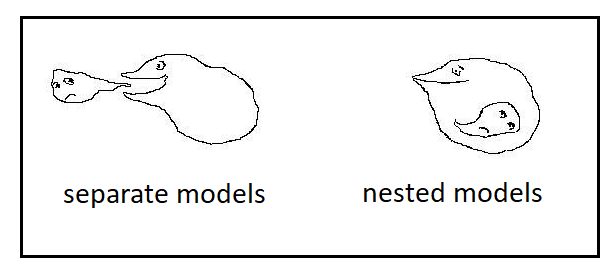
\includegraphics[width=0.5\textwidth]{images/AIC.png}
    \caption{Paveikslėlių numeriai rašomi apačioje, antraštė rašoma apačioje}
    \label{fig:grafikas1}
\end{figure}


Toliau eina tekstas po paveikslėliu.

\subsection{Sąrašai}

Nenumeruojamo sąrašo pavyzdys:
\begin{itemize}
    \item pirmasis elementas;
    \item antrasis elementas.
\end{itemize}

Numeruojamo sąrašo pavydzys:
\begin{enumerate}
    \item lorem ipsum dolor sit amet;
    \item consectetur adipiscing elit;
    \item vivamus a nisl gravida.
\end{enumerate}


\section{Programinio kodo pateikimas}
Šiame skyriuje pateikiamas programinio kodo pateikimo būdas rašto darbe.

\subsection{Algoritmai}

Algoritmai, lygiai taip pat, kaip ir paveikslėliai ar lentelės, yra numeruojami.
Juos būtina paminėti tekste, pvz.:~\ref{alg:gd} naudojamas surasti minimalią funkcijos $\mathcal{L}$ reikšmę.

\begin{algorithm}[h]
\caption{Gradientinio nusileidimo pseudokodas}\label{alg:gd}
\begin{algorithmic}[1]
    \STATE \textcolor{blue}{\texttt{\textbf{\# Darome prielaidą, kad $\mathcal{L}$ apibrėžtas tekste}}}
        \STATE Įeitis: $\mathcal{D}$ -- duomenų rinkinys
        \STATE Įeitis: $\theta_0$ -- parametrų atsitiktinių reikšmių inicializavimas
        \STATE Įeitis: $\gamma$ -- žingsnio dydis, mokymosi greitis (angl.~\textit{learning rate}, \textit{step size})
        \STATE Įeitis: $m$ -- epochų skaičius
        \FOR{$i = 1, 2, \dots, m$}
            \STATE $\theta_i \coloneq \theta_{i-1} - \gamma \nabla_\theta \mathcal{L}(\mathcal{D}, \theta_{i-1})$
            \STATE \textcolor{blue}{\texttt{\textbf{\# Funkcijos $\mathcal{L}$ išvestinė suskaičiuojama automatiškai, autograd pagalba}}}
        \ENDFOR
\end{algorithmic}
\end{algorithm}

\subsubsection{Skyrelio pavyzdys}
\noindent Nebūtina naudoti daug skyrelių (\textit{subsubsections}).

\sectionnonum{Rezultatai}
Detaliau, kas turi būti parašyta šiame skyriuje, rasite atitinkamos programos metodiniuose reikalavimuose. 

\sectionnonum{Išvados}
Detaliau, kas turi būti parašyta šiame skyriuje, rasite atitinkamos programos metodiniuose reikalavimuose. 

\printbibliography[title = {Šaltiniai}]


% \appendix
% \renewcommand{\thesection}{\arabic{section} priedas.}

% \section{\phantom{Priedas} Citavimo pavyzdžiai}
% Dokumente - \textit{bibliografija.bib}, reikia sudėti visus cituojamus šaltinius ir panaudojus funkciją \textit{\{\textbackslash cite\{cituojamo objekto pavadinimas\}\}} atitinkamas šaltinis bus pridėtas prie literatūros šaltinių sąrašo.


% \textit{bibliografija.bib} galima rasti kelių dažniausiai cituojamų šaltinių tipų pavyzdžius:
% \begin{itemize}
%     \item internetiniai puslapiai (\textit{@online}) \cite{PvzInternetinisPuslapis},
%     \item duomenų rinkiniai (\textit{@dataset}) \cite{dataset}
%     \item straipsniai (\textit{@article}) \cite{PvzStraipsnLt, PvzStraipsnEn}, 
%     \item straipsniai iš konferencijos (\textit{@inproceedings}) \cite{PvzKonfLt, PvzKonfEn}, 
%     \item knygos (\textit{@book}) \cite{PvzKnygLt, PvzKnygEn}, 
%     \item baigiamieji darbai (\textit{@thesis arba mastersthesis/phdthesis} \cite{PvzMagistrLt, PvzPhdEn})
%     \item elektroninės publikacijos (\textit{@misc}) \cite{PvzElPubLt, PvzElPubEn}
% \end{itemize}

% Taip pat yra pateikti pavyzdžiai - ChatGPT citavimui, tiek bendrai\cite{chatgpt_bendrai}, tiek konkrečiam pokalbiui\cite{chatgpt_pokalbis}.

\end{document}
